\documentclass[fleqn]{jbook}
\usepackage{physpub}
\usepackage{txfonts}

\begin{document}
\begin{question}{問題6}{三澤}
図1に示すように炭素イオン(荷電状態$q=+2$)が水素プラズマを通過するときの荷電状態の変化およびエネルギー損失を測定する実験を行った。炭素イオンの入射エネルギーは核子あたり350keV(速度は8.2$\times10^6$m/s)である。以下の設問に筋道を示して答えよ。必要であれば以下の値を用いよ。

炭素の質量数$A=12$、原子番号$Z=6$、光速度$3.0\times10^6$m/s、核子質量$m?n=1.7\times10^{-27}$kg、電荷単位$e=1.6\times10^{-19}$C。また、必要であれば$\exp(2.0)=7.4$の値を用いよ。

この実験において水素プラズマは陽子と電子に完全に電離し、それぞれの密度は空間的に一様で$n$であり、また時間的にも定常な状態であるとする。その厚さを$d$とする。
\begin{figure}[htbp]
\begin{center}
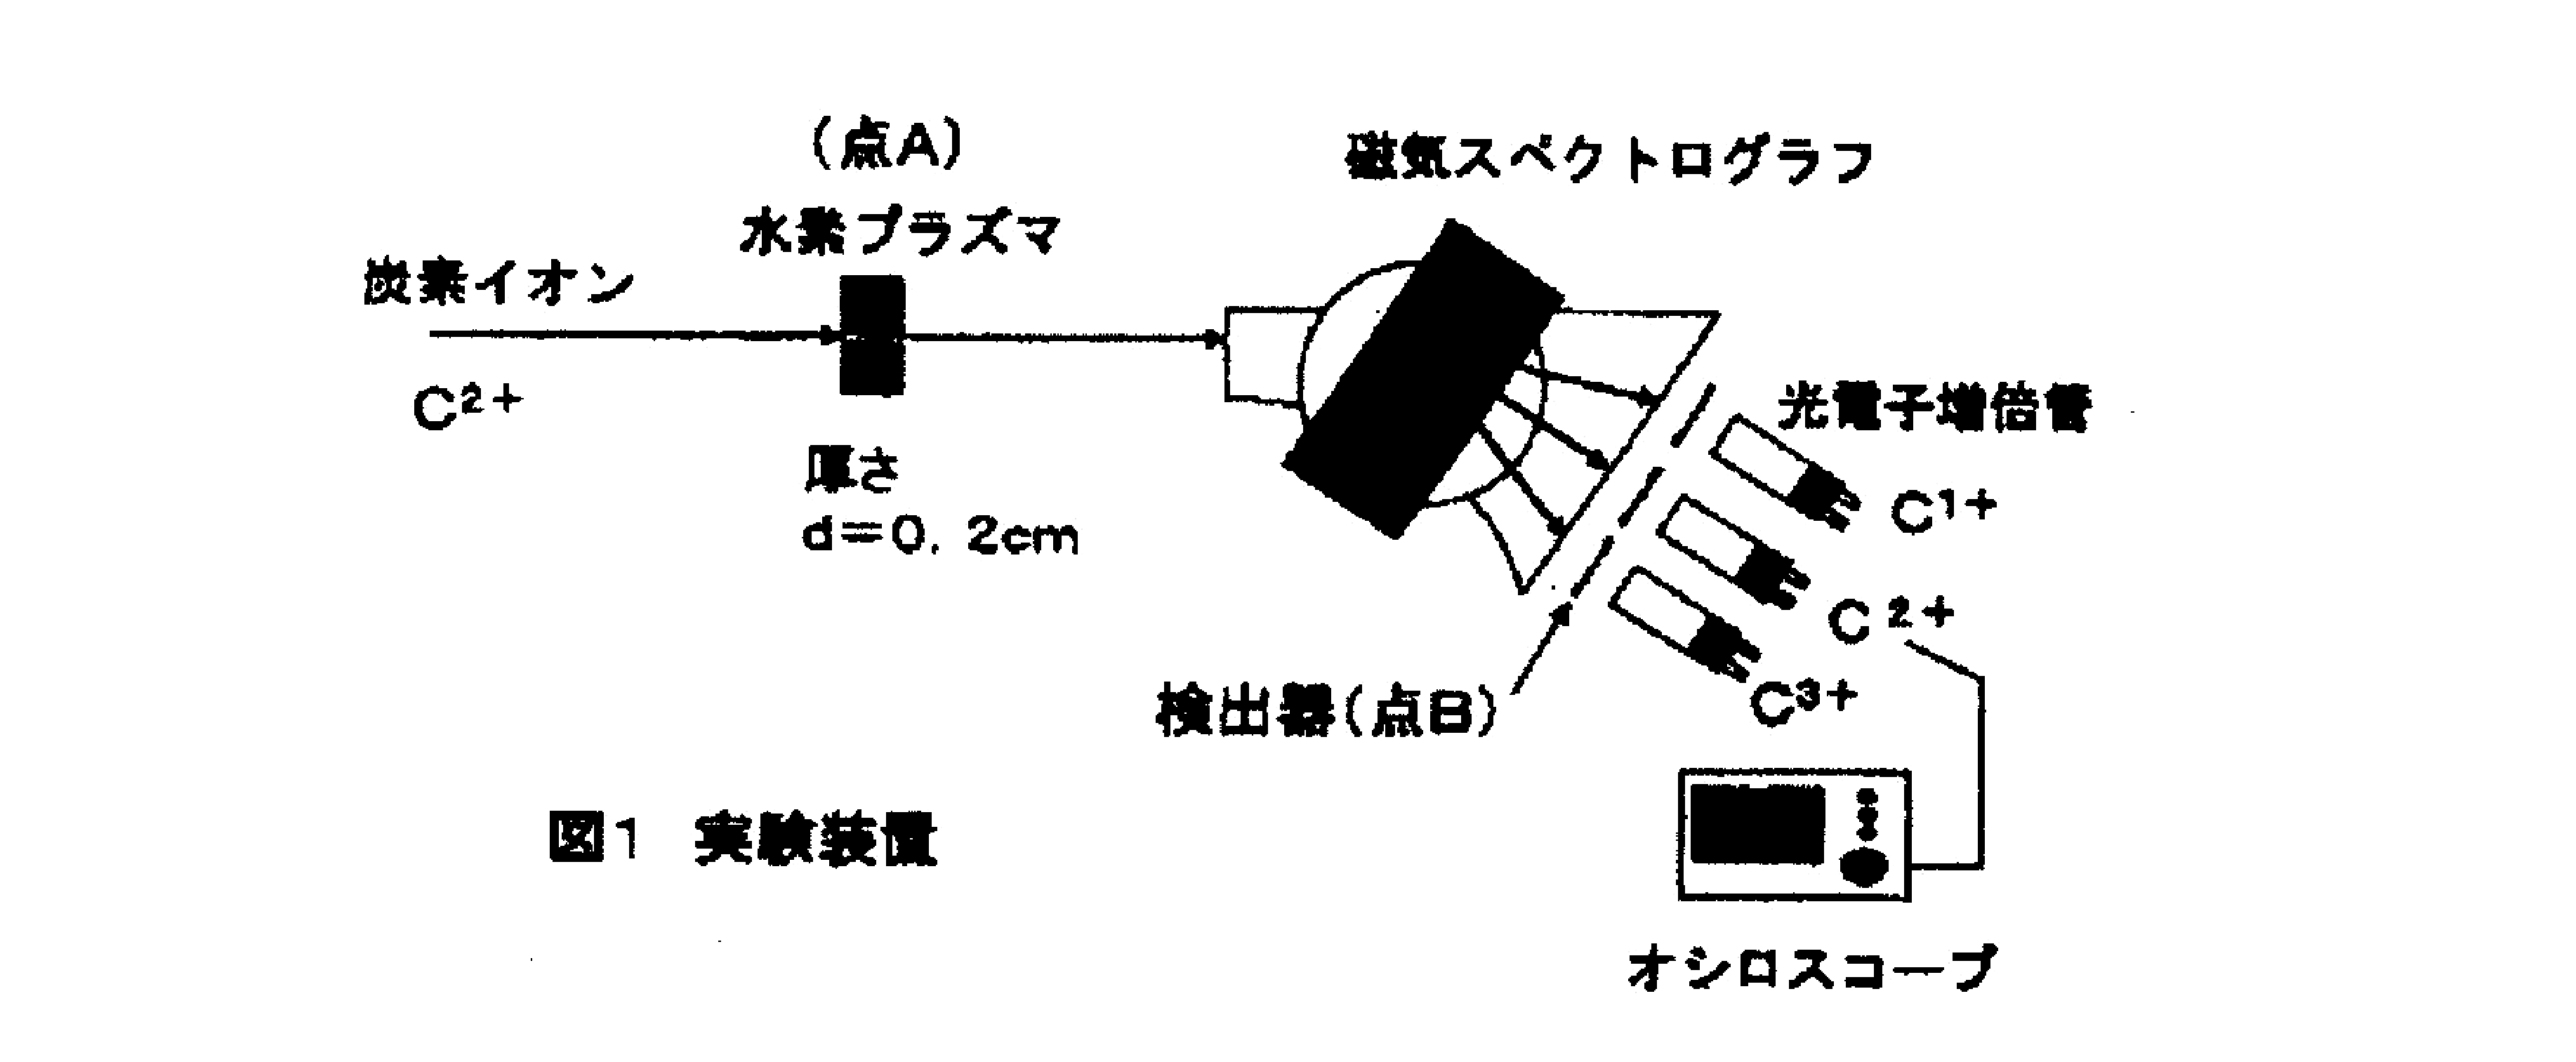
\includegraphics[width=.9\linewidth]{2002phy6q.eps}
\caption{実験装置}
\end{center}
\end{figure}
\begin{enumerate}
\item 炭素イオンは水素プラズマ内の陽子および自由電子と相互作用をして、電子が剥ぎ取られる電離と、自由電子を捕獲する再結合が行われ荷電状態が変化する。その反応断面積をそれぞれ$\sigma_i$、$\sigma_r$とする。これらの値は衝突のエネルギー、運動量によらないものとする。プラズマに$N_0$個の$q=+2$のイオンが入射されるとする。以下の設問において、一度変化した炭素イオンの荷電状態がさらに変化する現象は無視してよい。
\begin{enumerate}
\item プラズマ表面から炭素イオンの進む方向に向かっての距離を$x$とするとき($0\leq x\leq d$)、$x$の点で$q=+2$に留まっているイオンの数$N_2(x)$を表す式を求めよ。
\item イオンは再結合により$q=+1$、電離により$q=+3$、となるが、入射点から$x$までの間に生成される、それぞれのイオンの数$N_1(x)$、$N_3(x)$を表す式を求めよ。
\item $\sigma_i=1.0\times10^{-17}$cm$^2$、$\sigma_r=1.0\times10^{-22}$cm$^2$、$n=1\times10^{18}$cm$^{-3}$、$d=0.2$cmとする時、プラズマ通過後、荷電状態が$q=+1,+2,+3$状態となっている割合はいくらか。
\end{enumerate}
\item プラズマ通過後の荷電状態を調べるために図1に示すように磁気スペクトログラフ(図中で紙面に垂直に磁場をかけ、荷電粒子を曲げる装置)を用いて炭素イオンの荷電分布を調べた。スペクトログラフの磁束密度$B=0.1$T(ここでT=Wb/m$^2$)とする時、スペクトログラフ内での$q=+1,+2,+3$に対応する曲率半径$^rho_1,\rho_2,\rho_3$はいくらか。
\item 上記磁気スペクトログラフの磁場を測定したい。
\begin{enumerate}
\item 磁束密度の方向、つまりS極とN極を確かめたい。電池と針金を持ちいて確かめるにはどうすればよいか。図を描いて説明せよ。
\item 磁束密度$B$を測定する方法を一つあげ、その原理を簡単に説明せよ。
\end{enumerate}
\item プラズマ中でのイオンのエネルギー損失$\Delta E$を、プラズマでgち(図中の点A)から検出器(点B)までの飛行時間を測定して求める。プラズマが無いときとある時の飛行時間差$\Delta t$と$\Delta E$の関係式を求めよ。但し点Aから点Bまでの距離を$L_0$とする。$L_0=4$m、炭素イオンのエネルギーが核子あたり$E=350keV$の時、$\Delta t=5$ナノ秒であった。$\Delta E$はいくらになるか。
\item 前問において用いるイオン検出器として、プラスティックシンチレーター、NaIシンチレーターの2種類を用意した。上記の実験に用いるのはどちらのシンチレーターが適当であるかを理由を示して述べよ。
\end{enumerate}
\end{question}
\begin{answer}{問題6}{三澤}
\begin{enumerate}
\item
\begin{enumerate}
\item
$x+\triangle x$における $q=+2$のイオンの数を
$N_2(x+\triangle x)$とする。
ここで、
\begin{equation}
 \sigma = \sigma_i +\sigma_r
\end{equation}
とすると,
\begin{equation}
N_2(x+\triangle x)=N_2(x)-N_2(x)\times n\sigma\triangle x 
\end{equation}
となる。
これから、
\begin{equation}
 \frac{N_2(x+\triangle x)-N_2(x)}{\triangle x} = -N_2(x)\times n\sigma 
\end{equation}
となる。
$\triangle x\to0$として、

\begin{equation}
  \frac{dN_2(x)}{dx} = -n\sigma N_2(x) 
\end{equation}
をえる。$N_2(0)=N_0$を考慮してこの微分方程式の解は

\begin{equation}
N_2(x)=N_0\exp(-n\sigma x)
\end{equation}
となる。

\item
(i)と同様にして、
\begin{equation}
N_1(x+\triangle x)=N_1(x)+n\sigma_i N_2(x)\triangle x
\end{equation}
より、

\begin{equation}
\frac{dN_1(x)}{dx} = n\sigma N_2(x) 
\end{equation}
を得る。

ここで、$ N_2(x)=N_0\exp(-n\sigma x)$と、$N_1(0)=0$から、
この微分方程式の解は、

\begin{equation}
N_1(x)=\frac{\sigma_i}{\sigma}\times N_0\times (1-\exp(-n\sigma x) ) 
\end{equation}
である。

同様にして、

\begin{equation}
N_3(x)=\frac{\sigma_r}{\sigma}\times N_0\times (1-\exp(-n\sigma x) ) 
\end{equation}
をえる。

\item
$\sigma_i=1.0\times 10^{-17} cm^2,\sigma_r=1.0\times 10^{-22}cm^2,n=1\times 10^{16} cm^{-3},
d=0.2cm $である。よって、

\begin{equation}
 \begin{split}
   N_2(0.2)&=N_0\exp(-0.2\times n\times \sigma_i)\times \exp(-0.2\times n\times \sigma_r) \\
           &=N_0\exp(-2)\times \exp(-2\times 10^{-5}) \\
           &\approx N_0\exp(-2) \\
           &=N_0\times 1/7.4 
 \end{split}
\end{equation}
である。
また、

\begin{equation}
N_1(x)=\frac{\sigma_i}{\sigma}\times N_0\times (1-N_2(x))
\end{equation}
より、

\begin{equation}
 \begin{split}
  N_1(0.2)&=\frac{1.0\times 10^{-17} }{1.0\times 10^{-17} +1.0\times 10^{-22}}\times 
  N_0\times (1-N_2(0.2)) \\
          &\approx 1\times N_0\times (1-1/7.4) \\
          &=N_0\times 6.4/7.4
 \end{split}
\end{equation}
である。

同様に、


\begin{equation}
 N_3(x))=\frac{\sigma_r}{\sigma}\times N_0\times (1-N_2(x))
\end{equation}
より、

\begin{equation}
 \begin{split}
 N_3(0.2)&=\frac{1.0\times 10^{-22} }{1.0\times 10^{-17} +1.0\times 10^{-22}}\times 
 N_0\times (1-N_2(0.2)) \\
         &= \frac{1}{1+10^{5}}\times N_0\times (1-1/7.4) \\
         &\approx 10^{-5}\times N_0\times 6.4/7.4 \\
         &=N_0\times 6.4/7.4\times 10^{-5}
 \end{split}
\end{equation}
である。

以上から、
\begin{equation}
N_1(0.2):N_2(0.2):N_3(0.2) = 6.4:1:6.4\times 10^{-5}
\end{equation}
となる。
\end{enumerate}

\item
磁束密度$B$における、質量$m$、電荷$q$の粒子の曲率半径$\rho$は、

\begin{equation}
 m\frac{v^2}{\rho}=qvB
\end{equation}
より、

\begin{equation}
 \rho=\frac{mv}{qB}
\end{equation}
となる。ここで、

\begin{equation}
 m=12\times 1.7\times 10^{-27}
\end{equation}
である。よって、

\begin{equation}
 \begin{split}
  \rho_1&=\frac{20.4\times10^{-27}\times 8.2\times 10^{6} }{1\times 1.6\times 
10^{-19}\times 0.1} \\
   &=5.1\times 2.1 \\ 
   &=10.71\approx 11(m) 
 \end{split}
\end{equation}
である。
また、$\rho_2=\rho_1/2$より、

\begin{equation}
 \begin{split}
  \rho_2&=10.7/2 \\
        &=5.35 \\
        &\approx 5.4(m)
 \end{split}
\end{equation}
であり、同様に、$\rho_3=\rho_1/3$より、

\begin{equation}
 \begin{split}
  \rho_3&=10.7/3 \\
        &\approx 3.6(m)
 \end{split}
\end{equation}
である。
\item
\begin{enumerate}
\item~
\begin{minipage}{.7\linewidth}
右図の装置を用いて、
針金がどちらに動くかで
$B$の向きを決定する。
\end{minipage}
\begin{minipage}{.3\linewidth}
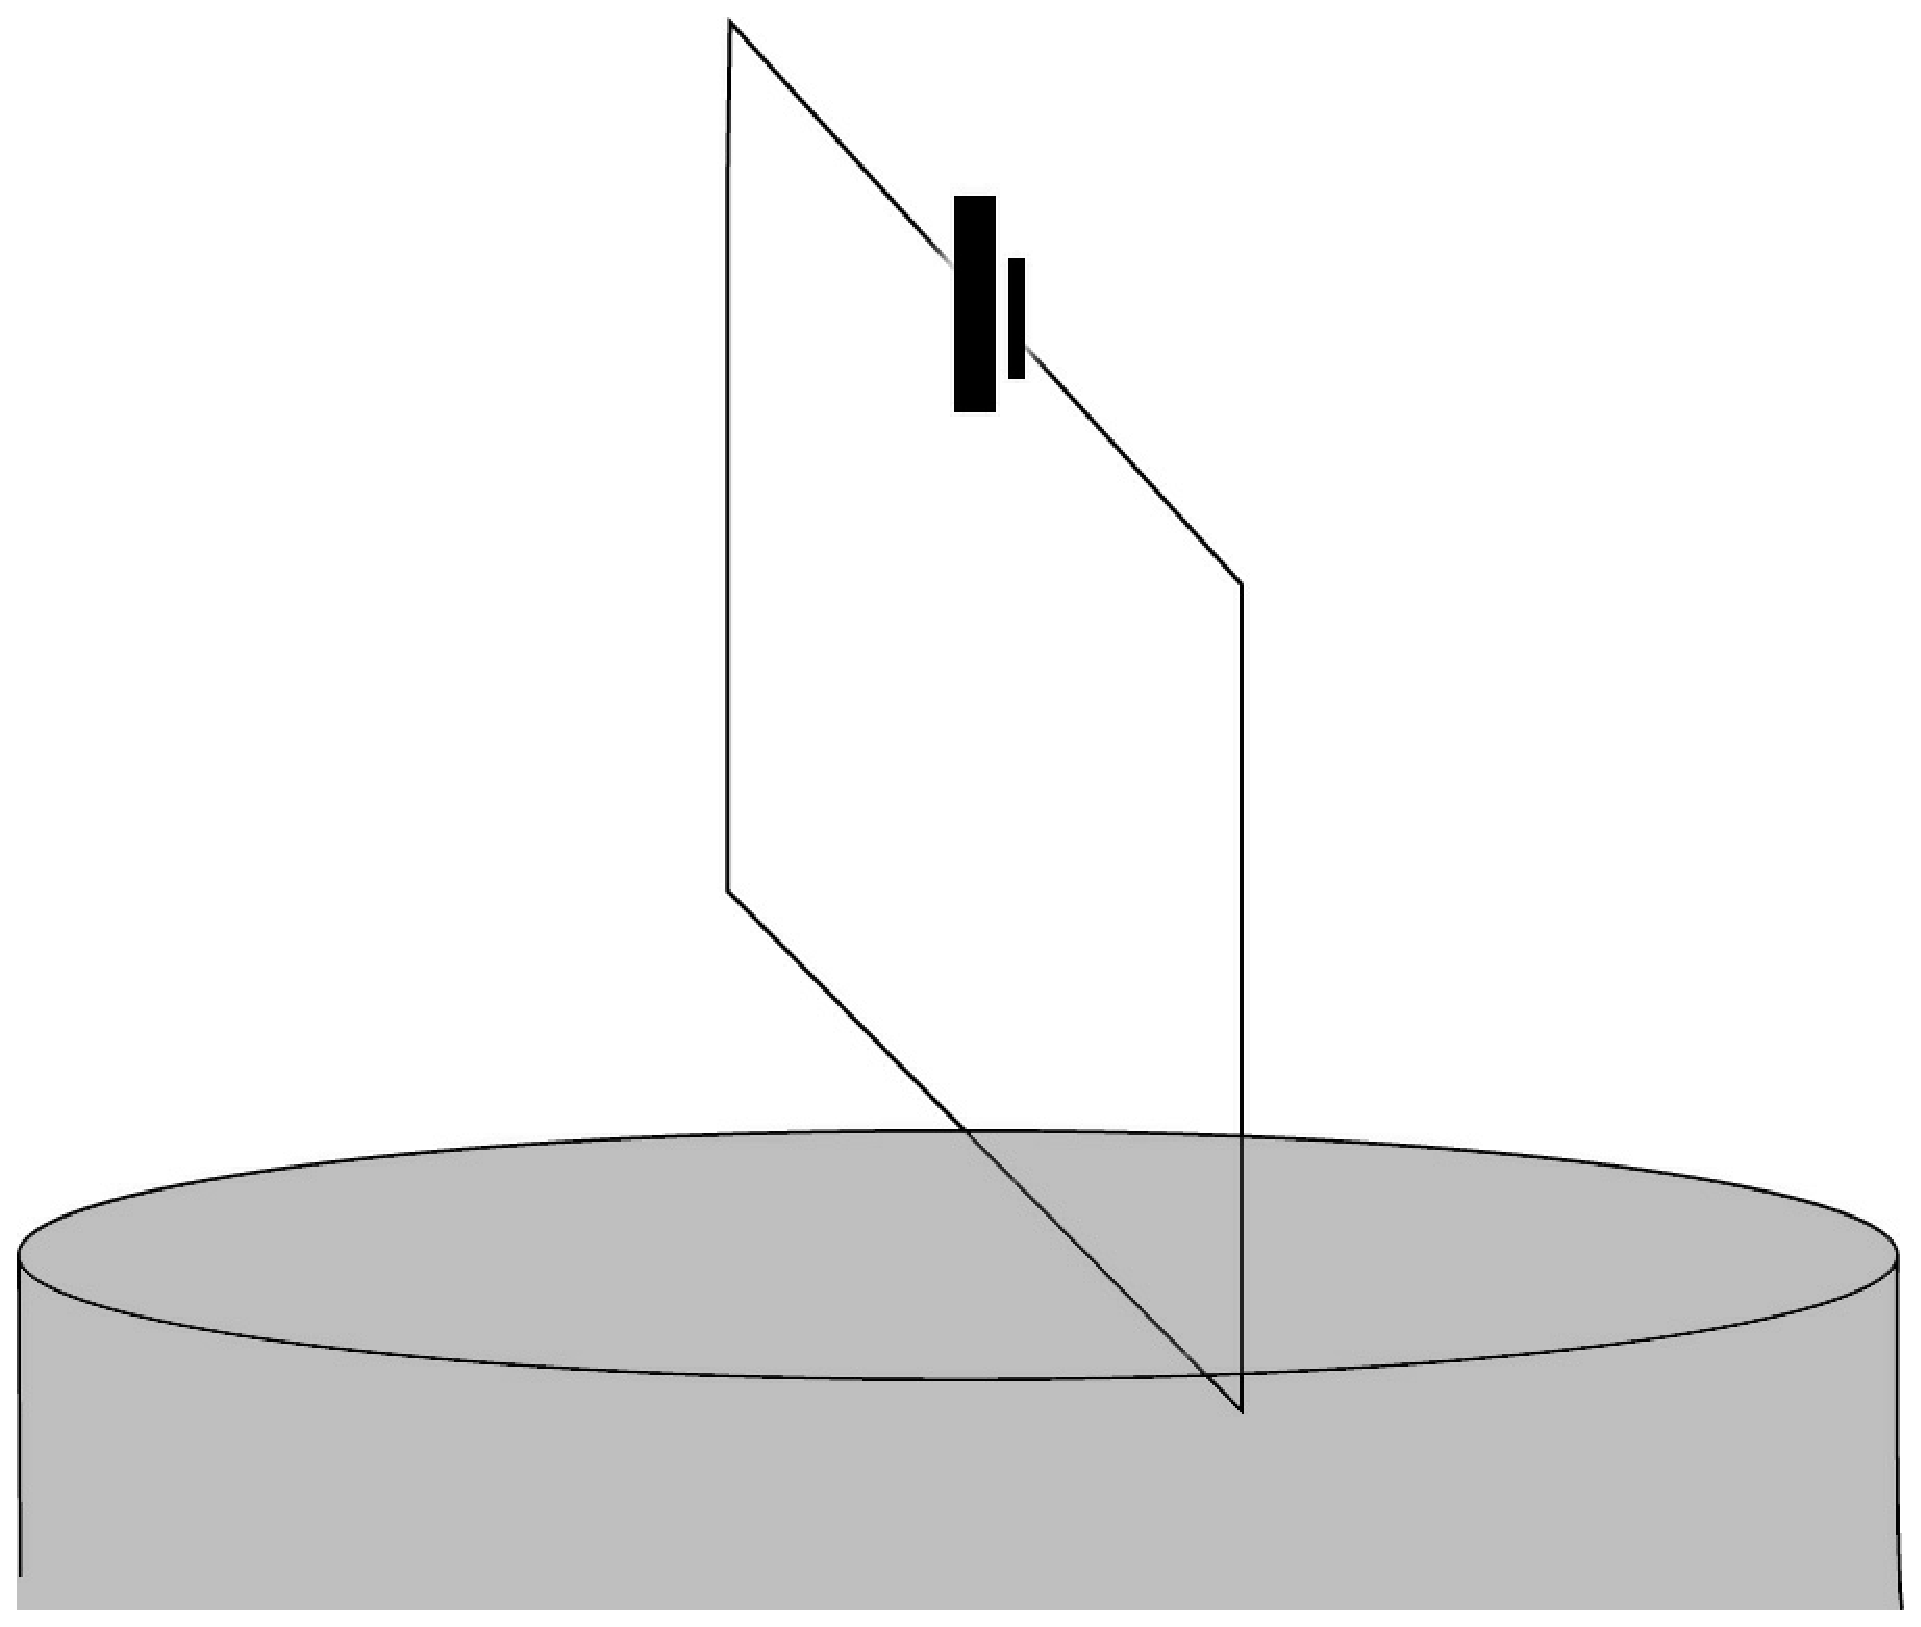
\includegraphics[width=\linewidth]{2002phy6a.eps}
\end{minipage}
\item
磁気モーメント$\bm{\mu}$を角運動量$\bm{J}=\hbar \bm{I}$を用いて、
$\bm{\mu}=\gamma \bm{J}$で定義する。これは静磁場$\bm{H}=\frac{\bm{B}}{\mu_0}$内では、
角速度$\bm{\omega}=-\gamma \bm{H}$で回転運動をする。この$\bm{\omega}$の大きさを測ることで、
磁場の大きさを決定する。
\end{enumerate}
\item
プラズマがない時の速度、エネルギーを$v_0$、$E_0$,ある時の速度、エネルギーを$v_1$とする。
すると、
\begin{equation}
\frac{1}{2}mv_0^2=E_0   
\end{equation}

\begin{equation}
\frac{1}{2}mv_1^2=E_0-\triangle E  
\end{equation}
となる。

これから、
\begin{equation}
\triangle E=\frac{1}{2}m\times (v_0^2-v_1^2) 
\end{equation}
である。
また、
\begin{equation}
\frac{L}{v_1}-\frac{L}{v_0}=t \Leftrightarrow  v_1=\frac{v_0L}{v_0\triangle t+L} 
\end{equation}
である。

(25),(26)から
\begin{equation}
\triangle E = \frac{1}{2}mv_0^2\times (1-\frac{L^2}{(v_0\triangle t+L)^2})
\end{equation}

値を代入して、

\begin{equation*}
 \begin{split}
 \triangle E &= 350\times ( 1-\frac{16}{ ( 4+8.2\times 5 \times 10^{-3})^{2}})\\
             &= 350\times ( 1-(1+10.25\times 10^{-3})^{-2} ) \\
             &= 350\times ( 1-(1-2\times 10.25\times 10^{-3}) )  \\
             &= 350\times 20.5\times 10^{-3} \\
             &= 7.175 
 \end{split}
\end{equation*}


よって、$\triangle E=7.2(keV)$である。 

\item
この実験のように、高速粒子の測定にはプラスティックシンチレーターのほうが向いている。
なぜなら、$NaI$シンチレーターは蛍光減衰時間がプラスティックシンチレーターに比べて、$100$
倍以上長くて、早い計測には向かないからである。
\end{enumerate}
\end{answer}
\end{document}
